\documentclass[1p]{elsarticle_modified}
%\bibliographystyle{elsarticle-num}

%\usepackage[colorlinks]{hyperref}
%\usepackage{abbrmath_seonhwa} %\Abb, \Ascr, \Acal ,\Abf, \Afrak
\usepackage{amsfonts}
\usepackage{amssymb}
\usepackage{amsmath}
\usepackage{amsthm}
\usepackage{scalefnt}
\usepackage{amsbsy}
\usepackage{kotex}
\usepackage{caption}
\usepackage{subfig}
\usepackage{color}
\usepackage{graphicx}
\usepackage{xcolor} %% white, black, red, green, blue, cyan, magenta, yellow
\usepackage{float}
\usepackage{setspace}
\usepackage{hyperref}

\usepackage{tikz}
\usetikzlibrary{arrows}

\usepackage{multirow}
\usepackage{array} % fixed length table
\usepackage{hhline}

%%%%%%%%%%%%%%%%%%%%%
\makeatletter
\renewcommand*\env@matrix[1][\arraystretch]{%
	\edef\arraystretch{#1}%
	\hskip -\arraycolsep
	\let\@ifnextchar\new@ifnextchar
	\array{*\c@MaxMatrixCols c}}
\makeatother %https://tex.stackexchange.com/questions/14071/how-can-i-increase-the-line-spacing-in-a-matrix
%%%%%%%%%%%%%%%

\usepackage[normalem]{ulem}

\newcommand{\msout}[1]{\ifmmode\text{\sout{\ensuremath{#1}}}\else\sout{#1}\fi}
%SOURCE: \msout is \stkout macro in https://tex.stackexchange.com/questions/20609/strikeout-in-math-mode

\newcommand{\cancel}[1]{
	\ifmmode
	{\color{red}\msout{#1}}
	\else
	{\color{red}\sout{#1}}
	\fi
}

\newcommand{\add}[1]{
	{\color{blue}\uwave{#1}}
}

\newcommand{\replace}[2]{
	\ifmmode
	{\color{red}\msout{#1}}{\color{blue}\uwave{#2}}
	\else
	{\color{red}\sout{#1}}{\color{blue}\uwave{#2}}
	\fi
}

\newcommand{\Sol}{\mathcal{S}} %segment
\newcommand{\D}{D} %diagram
\newcommand{\A}{\mathcal{A}} %arc


%%%%%%%%%%%%%%%%%%%%%%%%%%%%%5 test

\def\sl{\operatorname{\textup{SL}}(2,\Cbb)}
\def\psl{\operatorname{\textup{PSL}}(2,\Cbb)}
\def\quan{\mkern 1mu \triangleright \mkern 1mu}

\theoremstyle{definition}
\newtheorem{thm}{Theorem}[section]
\newtheorem{prop}[thm]{Proposition}
\newtheorem{lem}[thm]{Lemma}
\newtheorem{ques}[thm]{Question}
\newtheorem{cor}[thm]{Corollary}
\newtheorem{defn}[thm]{Definition}
\newtheorem{exam}[thm]{Example}
\newtheorem{rmk}[thm]{Remark}
\newtheorem{alg}[thm]{Algorithm}

\newcommand{\I}{\sqrt{-1}}
\begin{document}

%\begin{frontmatter}
%
%\title{Boundary parabolic representations of knots up to 8 crossings}
%
%%% Group authors per affiliation:
%\author{Yunhi Cho} 
%\address{Department of Mathematics, University of Seoul, Seoul, Korea}
%\ead{yhcho@uos.ac.kr}
%
%
%\author{Seonhwa Kim} %\fnref{s_kim}}
%\address{Center for Geometry and Physics, Institute for Basic Science, Pohang, 37673, Korea}
%\ead{ryeona17@ibs.re.kr}
%
%\author{Hyuk Kim}
%\address{Department of Mathematical Sciences, Seoul National University, Seoul 08826, Korea}
%\ead{hyukkim@snu.ac.kr}
%
%\author{Seokbeom Yoon}
%\address{Department of Mathematical Sciences, Seoul National University, Seoul, 08826,  Korea}
%\ead{sbyoon15@snu.ac.kr}
%
%\begin{abstract}
%We find all boundary parabolic representation of knots up to 8 crossings.
%
%\end{abstract}
%\begin{keyword}
%    \MSC[2010] 57M25 
%\end{keyword}
%
%\end{frontmatter}

%\linenumbers
%\tableofcontents
%
\newcommand\colored[1]{\textcolor{white}{\rule[-0.35ex]{0.8em}{1.4ex}}\kern-0.8em\color{red} #1}%
%\newcommand\colored[1]{\textcolor{white}{ #1}\kern-2.17ex	\textcolor{white}{ #1}\kern-1.81ex	\textcolor{white}{ #1}\kern-2.15ex\color{red}#1	}

{\Large $\underline{11a_{270}~(K11a_{270})}$}

\setlength{\tabcolsep}{10pt}
\renewcommand{\arraystretch}{1.6}
\vspace{1cm}\begin{tabular}{m{100pt}>{\centering\arraybackslash}m{274pt}}
\multirow{5}{120pt}{
	\centering
	\includegraphics[width=112pt]{../../../GIT/diagram.site/Diagrams/png/519_11a_270.png}\\
\ \ \ A knot diagram\footnotemark}&
\allowdisplaybreaks
\textbf{Linearized knot diagam} \\
\cline{2-2}
 &
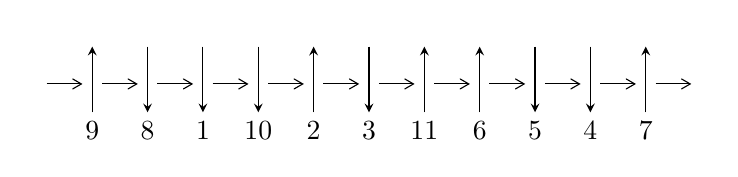
\begin{tikzpicture}[x=20pt, y=17pt]
	% nodes
	\node (C0) at (0, 0) {};
	\node (C1) at (1, 0) {};
	\node (C1U) at (1, +1) {};
	\node (C1D) at (1, -1) {9};

	\node (C2) at (2, 0) {};
	\node (C2U) at (2, +1) {};
	\node (C2D) at (2, -1) {8};

	\node (C3) at (3, 0) {};
	\node (C3U) at (3, +1) {};
	\node (C3D) at (3, -1) {1};

	\node (C4) at (4, 0) {};
	\node (C4U) at (4, +1) {};
	\node (C4D) at (4, -1) {10};

	\node (C5) at (5, 0) {};
	\node (C5U) at (5, +1) {};
	\node (C5D) at (5, -1) {2};

	\node (C6) at (6, 0) {};
	\node (C6U) at (6, +1) {};
	\node (C6D) at (6, -1) {3};

	\node (C7) at (7, 0) {};
	\node (C7U) at (7, +1) {};
	\node (C7D) at (7, -1) {11};

	\node (C8) at (8, 0) {};
	\node (C8U) at (8, +1) {};
	\node (C8D) at (8, -1) {6};

	\node (C9) at (9, 0) {};
	\node (C9U) at (9, +1) {};
	\node (C9D) at (9, -1) {5};

	\node (C10) at (10, 0) {};
	\node (C10U) at (10, +1) {};
	\node (C10D) at (10, -1) {4};

	\node (C11) at (11, 0) {};
	\node (C11U) at (11, +1) {};
	\node (C11D) at (11, -1) {7};
	\node (C12) at (12, 0) {};

	% arrows
	\draw[->,>={angle 60}]
	(C0) edge (C1) (C1) edge (C2) (C2) edge (C3) (C3) edge (C4) (C4) edge (C5) (C5) edge (C6) (C6) edge (C7) (C7) edge (C8) (C8) edge (C9) (C9) edge (C10) (C10) edge (C11) (C11) edge (C12) ;	\draw[->,>=stealth]
	(C1D) edge (C1U) (C2U) edge (C2D) (C3U) edge (C3D) (C4U) edge (C4D) (C5D) edge (C5U) (C6U) edge (C6D) (C7D) edge (C7U) (C8D) edge (C8U) (C9U) edge (C9D) (C10U) edge (C10D) (C11D) edge (C11U) ;
	\end{tikzpicture} \\
\hhline{~~} \\& 
\textbf{Solving Sequence} \\ \cline{2-2} 
 &
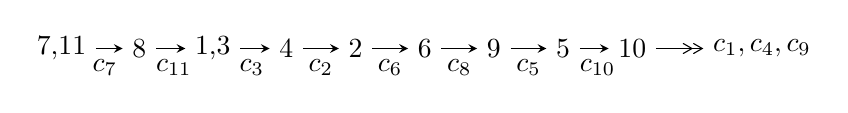
\begin{tikzpicture}[x=25pt, y=7pt]
	% node
	\node (A0) at (-1/8, 0) {7,11};
	\node (A1) at (1, 0) {8};
	\node (A2) at (33/16, 0) {1,3};
	\node (A3) at (25/8, 0) {4};
	\node (A4) at (33/8, 0) {2};
	\node (A5) at (41/8, 0) {6};
	\node (A6) at (49/8, 0) {9};
	\node (A7) at (57/8, 0) {5};
	\node (A8) at (65/8, 0) {10};
	\node (C1) at (1/2, -1) {$c_{7}$};
	\node (C2) at (3/2, -1) {$c_{11}$};
	\node (C3) at (21/8, -1) {$c_{3}$};
	\node (C4) at (29/8, -1) {$c_{2}$};
	\node (C5) at (37/8, -1) {$c_{6}$};
	\node (C6) at (45/8, -1) {$c_{8}$};
	\node (C7) at (53/8, -1) {$c_{5}$};
	\node (C8) at (61/8, -1) {$c_{10}$};
	\node (A9) at (10, 0) {$c_{1},c_{4},c_{9}$};

	% edge
	\draw[->,>=stealth]	
	(A0) edge (A1) (A1) edge (A2) (A2) edge (A3) (A3) edge (A4) (A4) edge (A5) (A5) edge (A6) (A6) edge (A7) (A7) edge (A8) ;
	\draw[->>,>={angle 60}]	
	(A8) edge (A9);
\end{tikzpicture} \\ 

\end{tabular} \\

\footnotetext{
The image of knot diagram is generated by the software ``\textbf{Draw programme}" developed by Andrew Bartholomew(\url{http://www.layer8.co.uk/maths/draw/index.htm\#Running-draw}), where we modified some parts for our purpose(\url{https://github.com/CATsTAILs/LinksPainter}).
}\phantom \\ \newline 
\centering \textbf{Ideals for irreducible components\footnotemark of $X_{\text{par}}$} 
 
\begin{align*}
I^u_{1}&=\langle 
6.22010\times10^{178} u^{84}-1.04877\times10^{178} u^{83}+\cdots+1.33787\times10^{178} b-2.94730\times10^{180},\\
\phantom{I^u_{1}}&\phantom{= \langle  }7.81629\times10^{180} u^{84}-4.66338\times10^{179} u^{83}+\cdots+1.19071\times10^{180} a-4.40124\times10^{182},\\
\phantom{I^u_{1}}&\phantom{= \langle  }u^{85}+22 u^{83}+\cdots+295 u-89\rangle \\
I^u_{2}&=\langle 
- u^{16}+u^{15}+\cdots+b-2 u,\;37 u^{16}-30 u^{15}+\cdots+3 a+35,\\
\phantom{I^u_{2}}&\phantom{= \langle  }u^{17}- u^{16}+4 u^{15}-4 u^{14}+6 u^{13}-7 u^{12}- u^{11}-16 u^9+19 u^8-27 u^7+33 u^6-22 u^5+24 u^4-8 u^3+8 u^2- u+1\rangle \\
\\
\end{align*}
\raggedright * 2 irreducible components of $\dim_{\mathbb{C}}=0$, with total 102 representations.\\
\footnotetext{All coefficients of polynomials are rational numbers. But the coefficients are sometimes approximated in decimal forms when there is not enough margin.}
\newpage
\renewcommand{\arraystretch}{1}
\centering \section*{I. $I^u_{1}= \langle 6.22\times10^{178} u^{84}-1.05\times10^{178} u^{83}+\cdots+1.34\times10^{178} b-2.95\times10^{180},\;7.82\times10^{180} u^{84}-4.66\times10^{179} u^{83}+\cdots+1.19\times10^{180} a-4.40\times10^{182},\;u^{85}+22 u^{83}+\cdots+295 u-89 \rangle$}
\flushleft \textbf{(i) Arc colorings}\\
\begin{tabular}{m{7pt} m{180pt} m{7pt} m{180pt} }
\flushright $a_{7}=$&$\begin{pmatrix}1\\0\end{pmatrix}$ \\
\flushright $a_{11}=$&$\begin{pmatrix}0\\u\end{pmatrix}$ \\
\flushright $a_{8}=$&$\begin{pmatrix}1\\- u^2\end{pmatrix}$ \\
\flushright $a_{1}=$&$\begin{pmatrix}u\\u\end{pmatrix}$ \\
\flushright $a_{3}=$&$\begin{pmatrix}-6.56441 u^{84}+0.391648 u^{83}+\cdots-695.862 u+369.633\\-4.64925 u^{84}+0.783909 u^{83}+\cdots-336.319 u+220.298\end{pmatrix}$ \\
\flushright $a_{4}=$&$\begin{pmatrix}-4.93046 u^{84}-0.281089 u^{83}+\cdots-750.595 u+334.722\\-3.01529 u^{84}+0.111172 u^{83}+\cdots-391.051 u+185.387\end{pmatrix}$ \\
\flushright $a_{2}=$&$\begin{pmatrix}-6.44414 u^{84}-1.95066 u^{83}+\cdots-1731.95 u+624.788\\-5.82573 u^{84}-0.575017 u^{83}+\cdots-1038.01 u+428.764\end{pmatrix}$ \\
\flushright $a_{6}=$&$\begin{pmatrix}18.3104 u^{84}-3.35235 u^{83}+\cdots+987.156 u-751.241\\14.6628 u^{84}-4.03186 u^{83}+\cdots+189.488 u-456.528\end{pmatrix}$ \\
\flushright $a_{9}=$&$\begin{pmatrix}14.7840 u^{84}+23.8120 u^{83}+\cdots+11886.5 u-3407.30\\13.1209 u^{84}+19.3511 u^{83}+\cdots+9780.17 u-2819.79\end{pmatrix}$ \\
\flushright $a_{5}=$&$\begin{pmatrix}26.1341 u^{84}-10.8653 u^{83}+\cdots-1474.91 u-346.013\\17.7162 u^{84}-10.4087 u^{83}+\cdots-2202.90 u+77.1428\end{pmatrix}$ \\
\flushright $a_{10}=$&$\begin{pmatrix}-1.61190 u^{84}+12.6221 u^{83}+\cdots+5431.09 u-1319.21\\0.891403 u^{84}+6.87910 u^{83}+\cdots+3129.32 u-802.311\end{pmatrix}$\\ \flushright $a_{10}=$&$\begin{pmatrix}-1.61190 u^{84}+12.6221 u^{83}+\cdots+5431.09 u-1319.21\\0.891403 u^{84}+6.87910 u^{83}+\cdots+3129.32 u-802.311\end{pmatrix}$\\&\end{tabular}
\flushleft \textbf{(ii) Obstruction class $= -1$}\\~\\
\flushleft \textbf{(iii) Cusp Shapes $= 10.9888 u^{84}-31.5549 u^{83}+\cdots-12310.5 u+2763.36$}\\~\\
\newpage\renewcommand{\arraystretch}{1}
\flushleft \textbf{(iv) u-Polynomials at the component}\newline \\
\begin{tabular}{m{50pt}|m{274pt}}
Crossings & \hspace{64pt}u-Polynomials at each crossing \\
\hline $$\begin{aligned}c_{1}\end{aligned}$$&$\begin{aligned}
&u^{85}-4 u^{84}+\cdots+405 u-83
\end{aligned}$\\
\hline $$\begin{aligned}c_{2}\end{aligned}$$&$\begin{aligned}
&u^{85}- u^{84}+\cdots-171 u-89
\end{aligned}$\\
\hline $$\begin{aligned}c_{3}\end{aligned}$$&$\begin{aligned}
&u^{85}+u^{84}+\cdots+172 u+28
\end{aligned}$\\
\hline $$\begin{aligned}c_{4},c_{9},c_{10}\end{aligned}$$&$\begin{aligned}
&u^{85}+u^{84}+\cdots+28 u-1
\end{aligned}$\\
\hline $$\begin{aligned}c_{5}\end{aligned}$$&$\begin{aligned}
&u^{85}-2 u^{84}+\cdots+2503 u+701
\end{aligned}$\\
\hline $$\begin{aligned}c_{6}\end{aligned}$$&$\begin{aligned}
&u^{85}-3 u^{84}+\cdots-216 u-47
\end{aligned}$\\
\hline $$\begin{aligned}c_{7},c_{11}\end{aligned}$$&$\begin{aligned}
&u^{85}+22 u^{83}+\cdots+295 u-89
\end{aligned}$\\
\hline $$\begin{aligned}c_{8}\end{aligned}$$&$\begin{aligned}
&u^{85}+6 u^{84}+\cdots-18 u-1
\end{aligned}$\\
\hline
\end{tabular}\\~\\
\newpage\renewcommand{\arraystretch}{1}
\flushleft \textbf{(v) Riley Polynomials at the component}\newline \\
\begin{tabular}{m{50pt}|m{274pt}}
Crossings & \hspace{64pt}Riley Polynomials at each crossing \\
\hline $$\begin{aligned}c_{1}\end{aligned}$$&$\begin{aligned}
&y^{85}-22 y^{84}+\cdots+57951 y-6889
\end{aligned}$\\
\hline $$\begin{aligned}c_{2}\end{aligned}$$&$\begin{aligned}
&y^{85}+5 y^{84}+\cdots-428219 y-7921
\end{aligned}$\\
\hline $$\begin{aligned}c_{3}\end{aligned}$$&$\begin{aligned}
&y^{85}- y^{84}+\cdots+36528 y-784
\end{aligned}$\\
\hline $$\begin{aligned}c_{4},c_{9},c_{10}\end{aligned}$$&$\begin{aligned}
&y^{85}+91 y^{84}+\cdots+108 y-1
\end{aligned}$\\
\hline $$\begin{aligned}c_{5}\end{aligned}$$&$\begin{aligned}
&y^{85}-26 y^{84}+\cdots+15305105 y-491401
\end{aligned}$\\
\hline $$\begin{aligned}c_{6}\end{aligned}$$&$\begin{aligned}
&y^{85}-27 y^{84}+\cdots-226978 y-2209
\end{aligned}$\\
\hline $$\begin{aligned}c_{7},c_{11}\end{aligned}$$&$\begin{aligned}
&y^{85}+44 y^{84}+\cdots-152029 y-7921
\end{aligned}$\\
\hline $$\begin{aligned}c_{8}\end{aligned}$$&$\begin{aligned}
&y^{85}+14 y^{84}+\cdots-46 y-1
\end{aligned}$\\
\hline
\end{tabular}\\~\\
\newpage\flushleft \textbf{(vi) Complex Volumes and Cusp Shapes}
$$\begin{array}{c|c|c}  
\text{Solutions to }I^u_{1}& \I (\text{vol} + \sqrt{-1}CS) & \text{Cusp shape}\\
 \hline 
\begin{aligned}
u &= -0.990583 + 0.156780 I \\
a &= -0.010000 - 0.290185 I \\
b &= \phantom{-}0.910228 - 0.729936 I\end{aligned}
 & \phantom{-}0.50703 + 7.20249 I & \phantom{-0.000000 } 0 \\ \hline\begin{aligned}
u &= -0.990583 - 0.156780 I \\
a &= -0.010000 + 0.290185 I \\
b &= \phantom{-}0.910228 + 0.729936 I\end{aligned}
 & \phantom{-}0.50703 - 7.20249 I & \phantom{-0.000000 } 0 \\ \hline\begin{aligned}
u &= \phantom{-}0.348189 + 0.949764 I \\
a &= -0.299627 - 0.451517 I \\
b &= \phantom{-}0.343573 + 1.260330 I\end{aligned}
 & \phantom{-}5.97217 - 3.17989 I & \phantom{-0.000000 } 0 \\ \hline\begin{aligned}
u &= \phantom{-}0.348189 - 0.949764 I \\
a &= -0.299627 + 0.451517 I \\
b &= \phantom{-}0.343573 - 1.260330 I\end{aligned}
 & \phantom{-}5.97217 + 3.17989 I & \phantom{-0.000000 } 0 \\ \hline\begin{aligned}
u &= -0.826847 + 0.527088 I \\
a &= -1.26230 + 0.66261 I \\
b &= -0.805769 - 0.073598 I\end{aligned}
 & \phantom{-}7.26328 - 2.81966 I & \phantom{-0.000000 } 0 \\ \hline\begin{aligned}
u &= -0.826847 - 0.527088 I \\
a &= -1.26230 - 0.66261 I \\
b &= -0.805769 + 0.073598 I\end{aligned}
 & \phantom{-}7.26328 + 2.81966 I & \phantom{-0.000000 } 0 \\ \hline\begin{aligned}
u &= -0.504249 + 0.900938 I \\
a &= -0.495942 - 0.147918 I \\
b &= -0.175068 + 0.862462 I\end{aligned}
 & \phantom{-}6.60839 - 2.04669 I & \phantom{-0.000000 } 0 \\ \hline\begin{aligned}
u &= -0.504249 - 0.900938 I \\
a &= -0.495942 + 0.147918 I \\
b &= -0.175068 - 0.862462 I\end{aligned}
 & \phantom{-}6.60839 + 2.04669 I & \phantom{-0.000000 } 0 \\ \hline\begin{aligned}
u &= \phantom{-}0.370751 + 0.964511 I \\
a &= \phantom{-}2.09678 + 0.74849 I \\
b &= \phantom{-}1.78001 - 0.38010 I\end{aligned}
 & -1.29284 + 1.77043 I & \phantom{-0.000000 } 0 \\ \hline\begin{aligned}
u &= \phantom{-}0.370751 - 0.964511 I \\
a &= \phantom{-}2.09678 - 0.74849 I \\
b &= \phantom{-}1.78001 + 0.38010 I\end{aligned}
 & -1.29284 - 1.77043 I & \phantom{-0.000000 } 0\\
 \hline 
 \end{array}$$\newpage$$\begin{array}{c|c|c}  
\text{Solutions to }I^u_{1}& \I (\text{vol} + \sqrt{-1}CS) & \text{Cusp shape}\\
 \hline 
\begin{aligned}
u &= -0.121508 + 1.029770 I \\
a &= -1.44704 + 0.90742 I \\
b &= -1.006470 - 0.378372 I\end{aligned}
 & -3.93614 - 0.79985 I & \phantom{-0.000000 } 0 \\ \hline\begin{aligned}
u &= -0.121508 - 1.029770 I \\
a &= -1.44704 - 0.90742 I \\
b &= -1.006470 + 0.378372 I\end{aligned}
 & -3.93614 + 0.79985 I & \phantom{-0.000000 } 0 \\ \hline\begin{aligned}
u &= -0.532279 + 0.762499 I \\
a &= -1.46595 - 0.28104 I \\
b &= -0.0316121 + 0.1122330 I\end{aligned}
 & \phantom{-}7.05028 - 2.25316 I & \phantom{-0.000000 } 0 \\ \hline\begin{aligned}
u &= -0.532279 - 0.762499 I \\
a &= -1.46595 + 0.28104 I \\
b &= -0.0316121 - 0.1122330 I\end{aligned}
 & \phantom{-}7.05028 + 2.25316 I & \phantom{-0.000000 } 0 \\ \hline\begin{aligned}
u &= -0.251015 + 1.055200 I \\
a &= -2.11732 - 0.34070 I \\
b &= -0.701200 - 0.509768 I\end{aligned}
 & -0.68905 - 4.95944 I & \phantom{-0.000000 } 0 \\ \hline\begin{aligned}
u &= -0.251015 - 1.055200 I \\
a &= -2.11732 + 0.34070 I \\
b &= -0.701200 + 0.509768 I\end{aligned}
 & -0.68905 + 4.95944 I & \phantom{-0.000000 } 0 \\ \hline\begin{aligned}
u &= -0.290713 + 0.867463 I \\
a &= \phantom{-}1.38286 - 0.59197 I \\
b &= \phantom{-}1.28028 - 1.10864 I\end{aligned}
 & \phantom{-}5.29095 - 1.80419 I & \phantom{-0.000000 } 0 \\ \hline\begin{aligned}
u &= -0.290713 - 0.867463 I \\
a &= \phantom{-}1.38286 + 0.59197 I \\
b &= \phantom{-}1.28028 + 1.10864 I\end{aligned}
 & \phantom{-}5.29095 + 1.80419 I & \phantom{-0.000000 } 0 \\ \hline\begin{aligned}
u &= -0.270696 + 0.871703 I \\
a &= \phantom{-}2.72325 + 0.14432 I \\
b &= \phantom{-}1.54169 + 0.09691 I\end{aligned}
 & \phantom{-}5.31835 - 0.73098 I & \phantom{-0.000000 } 0 \\ \hline\begin{aligned}
u &= -0.270696 - 0.871703 I \\
a &= \phantom{-}2.72325 - 0.14432 I \\
b &= \phantom{-}1.54169 - 0.09691 I\end{aligned}
 & \phantom{-}5.31835 + 0.73098 I & \phantom{-0.000000 } 0\\
 \hline 
 \end{array}$$\newpage$$\begin{array}{c|c|c}  
\text{Solutions to }I^u_{1}& \I (\text{vol} + \sqrt{-1}CS) & \text{Cusp shape}\\
 \hline 
\begin{aligned}
u &= \phantom{-}0.476405 + 0.979571 I \\
a &= \phantom{-}0.020053 - 0.849554 I \\
b &= -0.55978 - 1.60625 I\end{aligned}
 & \phantom{-}6.89508 + 8.42993 I & \phantom{-0.000000 } 0 \\ \hline\begin{aligned}
u &= \phantom{-}0.476405 - 0.979571 I \\
a &= \phantom{-}0.020053 + 0.849554 I \\
b &= -0.55978 + 1.60625 I\end{aligned}
 & \phantom{-}6.89508 - 8.42993 I & \phantom{-0.000000 } 0 \\ \hline\begin{aligned}
u &= -0.251627 + 0.867975 I \\
a &= \phantom{-}1.72706 + 0.60350 I \\
b &= \phantom{-}0.898499 + 0.920377 I\end{aligned}
 & \phantom{-}0.47607 + 1.35841 I & \phantom{-0.000000 } 0 \\ \hline\begin{aligned}
u &= -0.251627 - 0.867975 I \\
a &= \phantom{-}1.72706 - 0.60350 I \\
b &= \phantom{-}0.898499 - 0.920377 I\end{aligned}
 & \phantom{-}0.47607 - 1.35841 I & \phantom{-0.000000 } 0 \\ \hline\begin{aligned}
u &= \phantom{-}0.867924 + 0.117197 I \\
a &= \phantom{-}0.401814 - 0.078087 I \\
b &= \phantom{-}0.073704 - 0.631355 I\end{aligned}
 & \phantom{-}2.45654 + 0.38545 I & \phantom{-0.000000 } 0 \\ \hline\begin{aligned}
u &= \phantom{-}0.867924 - 0.117197 I \\
a &= \phantom{-}0.401814 + 0.078087 I \\
b &= \phantom{-}0.073704 + 0.631355 I\end{aligned}
 & \phantom{-}2.45654 - 0.38545 I & \phantom{-0.000000 } 0 \\ \hline\begin{aligned}
u &= -0.511179 + 1.033880 I \\
a &= -0.860377 + 0.932551 I \\
b &= -1.197380 - 0.080280 I\end{aligned}
 & -3.67030 - 1.93800 I & \phantom{-0.000000 } 0 \\ \hline\begin{aligned}
u &= -0.511179 - 1.033880 I \\
a &= -0.860377 - 0.932551 I \\
b &= -1.197380 + 0.080280 I\end{aligned}
 & -3.67030 + 1.93800 I & \phantom{-0.000000 } 0 \\ \hline\begin{aligned}
u &= \phantom{-}0.804514 + 0.199840 I \\
a &= -0.254918 - 0.463753 I \\
b &= \phantom{-}0.861149 + 0.863904 I\end{aligned}
 & \phantom{-}4.16809 - 3.00834 I & \phantom{-0.000000 } 0 \\ \hline\begin{aligned}
u &= \phantom{-}0.804514 - 0.199840 I \\
a &= -0.254918 + 0.463753 I \\
b &= \phantom{-}0.861149 - 0.863904 I\end{aligned}
 & \phantom{-}4.16809 + 3.00834 I & \phantom{-0.000000 } 0\\
 \hline 
 \end{array}$$\newpage$$\begin{array}{c|c|c}  
\text{Solutions to }I^u_{1}& \I (\text{vol} + \sqrt{-1}CS) & \text{Cusp shape}\\
 \hline 
\begin{aligned}
u &= \phantom{-}0.224344 + 0.788625 I \\
a &= \phantom{-}3.65794 - 0.56435 I \\
b &= \phantom{-}0.411602 - 0.536484 I\end{aligned}
 & \phantom{-}6.72774 + 5.81245 I & \phantom{-0.000000 } 0. - 10.65615 I \\ \hline\begin{aligned}
u &= \phantom{-}0.224344 - 0.788625 I \\
a &= \phantom{-}3.65794 + 0.56435 I \\
b &= \phantom{-}0.411602 + 0.536484 I\end{aligned}
 & \phantom{-}6.72774 - 5.81245 I & \phantom{-0.000000 -}0. + 10.65615 I \\ \hline\begin{aligned}
u &= \phantom{-}1.151880 + 0.340683 I \\
a &= -0.125453 - 0.215082 I \\
b &= -1.039420 - 0.763839 I\end{aligned}
 & \phantom{-}7.27474 - 10.59070 I & \phantom{-0.000000 } 0 \\ \hline\begin{aligned}
u &= \phantom{-}1.151880 - 0.340683 I \\
a &= -0.125453 + 0.215082 I \\
b &= -1.039420 + 0.763839 I\end{aligned}
 & \phantom{-}7.27474 + 10.59070 I & \phantom{-0.000000 } 0 \\ \hline\begin{aligned}
u &= -0.451547 + 1.119340 I \\
a &= -1.83462 + 0.36797 I \\
b &= -1.37742 - 0.92532 I\end{aligned}
 & -3.81248 - 5.22210 I & \phantom{-0.000000 } 0 \\ \hline\begin{aligned}
u &= -0.451547 - 1.119340 I \\
a &= -1.83462 - 0.36797 I \\
b &= -1.37742 + 0.92532 I\end{aligned}
 & -3.81248 + 5.22210 I & \phantom{-0.000000 } 0 \\ \hline\begin{aligned}
u &= -0.261477 + 0.747690 I \\
a &= -0.432549 - 1.141910 I \\
b &= \phantom{-}0.03198 - 1.67566 I\end{aligned}
 & \phantom{-}0.88272 - 4.07370 I & \phantom{-0.000000 -}0. + 10.38748 I \\ \hline\begin{aligned}
u &= -0.261477 - 0.747690 I \\
a &= -0.432549 + 1.141910 I \\
b &= \phantom{-}0.03198 + 1.67566 I\end{aligned}
 & \phantom{-}0.88272 + 4.07370 I & \phantom{-0.000000 } 0. - 10.38748 I \\ \hline\begin{aligned}
u &= \phantom{-}0.282937 + 1.182750 I \\
a &= \phantom{-}1.022110 + 0.688758 I \\
b &= \phantom{-}1.125510 + 0.384277 I\end{aligned}
 & -0.241277 + 0.561006 I & \phantom{-0.000000 } 0 \\ \hline\begin{aligned}
u &= \phantom{-}0.282937 - 1.182750 I \\
a &= \phantom{-}1.022110 - 0.688758 I \\
b &= \phantom{-}1.125510 - 0.384277 I\end{aligned}
 & -0.241277 - 0.561006 I & \phantom{-0.000000 } 0\\
 \hline 
 \end{array}$$\newpage$$\begin{array}{c|c|c}  
\text{Solutions to }I^u_{1}& \I (\text{vol} + \sqrt{-1}CS) & \text{Cusp shape}\\
 \hline 
\begin{aligned}
u &= \phantom{-}0.289715 + 0.708348 I \\
a &= \phantom{-}0.642373 + 0.547818 I \\
b &= \phantom{-}0.358840 + 0.533193 I\end{aligned}
 & -0.10663 + 1.41201 I & \phantom{-0.000000 } 0. - 4.19142 I \\ \hline\begin{aligned}
u &= \phantom{-}0.289715 - 0.708348 I \\
a &= \phantom{-}0.642373 - 0.547818 I \\
b &= \phantom{-}0.358840 - 0.533193 I\end{aligned}
 & -0.10663 - 1.41201 I & \phantom{-0.000000 -}0. + 4.19142 I \\ \hline\begin{aligned}
u &= \phantom{-}0.772781 + 0.972939 I \\
a &= \phantom{-}0.563431 + 0.899223 I \\
b &= \phantom{-}1.392510 - 0.236188 I\end{aligned}
 & \phantom{-}1.25410 + 3.01463 I & \phantom{-0.000000 } 0 \\ \hline\begin{aligned}
u &= \phantom{-}0.772781 - 0.972939 I \\
a &= \phantom{-}0.563431 - 0.899223 I \\
b &= \phantom{-}1.392510 + 0.236188 I\end{aligned}
 & \phantom{-}1.25410 - 3.01463 I & \phantom{-0.000000 } 0 \\ \hline\begin{aligned}
u &= \phantom{-}0.405461 + 1.174790 I \\
a &= -1.92488 + 0.10074 I \\
b &= -1.51977 + 0.86693 I\end{aligned}
 & -3.19196 + 6.54059 I & \phantom{-0.000000 } 0 \\ \hline\begin{aligned}
u &= \phantom{-}0.405461 - 1.174790 I \\
a &= -1.92488 - 0.10074 I \\
b &= -1.51977 - 0.86693 I\end{aligned}
 & -3.19196 - 6.54059 I & \phantom{-0.000000 } 0 \\ \hline\begin{aligned}
u &= \phantom{-}0.283503 + 1.211850 I \\
a &= \phantom{-}1.23366 + 0.88279 I \\
b &= \phantom{-}0.781274 - 0.343663 I\end{aligned}
 & -4.50297 + 4.26915 I & \phantom{-0.000000 } 0 \\ \hline\begin{aligned}
u &= \phantom{-}0.283503 - 1.211850 I \\
a &= \phantom{-}1.23366 - 0.88279 I \\
b &= \phantom{-}0.781274 + 0.343663 I\end{aligned}
 & -4.50297 - 4.26915 I & \phantom{-0.000000 } 0 \\ \hline\begin{aligned}
u &= \phantom{-}1.24666\phantom{ +0.000000I} \\
a &= \phantom{-}0.301059\phantom{ +0.000000I} \\
b &= \phantom{-}0.416139\phantom{ +0.000000I}\end{aligned}
 & \phantom{-}2.46366\phantom{ +0.000000I} & \phantom{-0.000000 } 0 \\ \hline\begin{aligned}
u &= \phantom{-}0.483671 + 0.546181 I \\
a &= -2.58654 - 0.36620 I \\
b &= -0.779143 + 0.909707 I\end{aligned}
 & \phantom{-}8.18862 - 4.43585 I & \phantom{-}5.12877 + 0. I\phantom{ +0.000000I}\\
 \hline 
 \end{array}$$\newpage$$\begin{array}{c|c|c}  
\text{Solutions to }I^u_{1}& \I (\text{vol} + \sqrt{-1}CS) & \text{Cusp shape}\\
 \hline 
\begin{aligned}
u &= \phantom{-}0.483671 - 0.546181 I \\
a &= -2.58654 + 0.36620 I \\
b &= -0.779143 - 0.909707 I\end{aligned}
 & \phantom{-}8.18862 + 4.43585 I & \phantom{-}5.12877 + 0. I\phantom{ +0.000000I} \\ \hline\begin{aligned}
u &= \phantom{-}0.531255 + 1.172220 I \\
a &= \phantom{-}1.68589 + 0.40460 I \\
b &= \phantom{-}1.08577 - 1.17737 I\end{aligned}
 & \phantom{-}1.30376 + 7.93201 I & \phantom{-0.000000 } 0 \\ \hline\begin{aligned}
u &= \phantom{-}0.531255 - 1.172220 I \\
a &= \phantom{-}1.68589 - 0.40460 I \\
b &= \phantom{-}1.08577 + 1.17737 I\end{aligned}
 & \phantom{-}1.30376 - 7.93201 I & \phantom{-0.000000 } 0 \\ \hline\begin{aligned}
u &= \phantom{-}0.470292 + 1.198160 I \\
a &= -1.090840 + 0.207986 I \\
b &= -0.837680 + 0.961854 I\end{aligned}
 & -0.82206 + 4.30776 I & \phantom{-0.000000 } 0 \\ \hline\begin{aligned}
u &= \phantom{-}0.470292 - 1.198160 I \\
a &= -1.090840 - 0.207986 I \\
b &= -0.837680 - 0.961854 I\end{aligned}
 & -0.82206 - 4.30776 I & \phantom{-0.000000 } 0 \\ \hline\begin{aligned}
u &= -1.184660 + 0.505149 I \\
a &= -0.169952 - 0.204856 I \\
b &= \phantom{-}0.530026 - 0.504262 I\end{aligned}
 & \phantom{-}8.34857 + 2.37496 I & \phantom{-0.000000 } 0 \\ \hline\begin{aligned}
u &= -1.184660 - 0.505149 I \\
a &= -0.169952 + 0.204856 I \\
b &= \phantom{-}0.530026 + 0.504262 I\end{aligned}
 & \phantom{-}8.34857 - 2.37496 I & \phantom{-0.000000 } 0 \\ \hline\begin{aligned}
u &= \phantom{-}0.573453 + 1.187210 I \\
a &= -0.255978 - 0.616026 I \\
b &= -0.567825 + 0.210292 I\end{aligned}
 & -2.13717 + 1.86843 I & \phantom{-0.000000 } 0 \\ \hline\begin{aligned}
u &= \phantom{-}0.573453 - 1.187210 I \\
a &= -0.255978 + 0.616026 I \\
b &= -0.567825 - 0.210292 I\end{aligned}
 & -2.13717 - 1.86843 I & \phantom{-0.000000 } 0 \\ \hline\begin{aligned}
u &= -0.281772 + 1.330610 I \\
a &= \phantom{-}0.791575 - 0.657737 I \\
b &= \phantom{-}0.774412 + 0.043237 I\end{aligned}
 & -4.64818 + 2.67744 I & \phantom{-0.000000 } 0\\
 \hline 
 \end{array}$$\newpage$$\begin{array}{c|c|c}  
\text{Solutions to }I^u_{1}& \I (\text{vol} + \sqrt{-1}CS) & \text{Cusp shape}\\
 \hline 
\begin{aligned}
u &= -0.281772 - 1.330610 I \\
a &= \phantom{-}0.791575 + 0.657737 I \\
b &= \phantom{-}0.774412 - 0.043237 I\end{aligned}
 & -4.64818 - 2.67744 I & \phantom{-0.000000 } 0 \\ \hline\begin{aligned}
u &= -0.553567 + 1.250070 I \\
a &= \phantom{-}1.70321 - 0.18110 I \\
b &= \phantom{-}1.41016 + 0.89938 I\end{aligned}
 & -2.87315 - 12.69490 I & \phantom{-0.000000 } 0 \\ \hline\begin{aligned}
u &= -0.553567 - 1.250070 I \\
a &= \phantom{-}1.70321 + 0.18110 I \\
b &= \phantom{-}1.41016 - 0.89938 I\end{aligned}
 & -2.87315 + 12.69490 I & \phantom{-0.000000 } 0 \\ \hline\begin{aligned}
u &= -0.399494 + 1.309870 I \\
a &= -1.22949 + 0.92957 I \\
b &= -0.642917 - 0.341349 I\end{aligned}
 & \phantom{-}1.87995 - 6.80929 I & \phantom{-0.000000 } 0 \\ \hline\begin{aligned}
u &= -0.399494 - 1.309870 I \\
a &= -1.22949 - 0.92957 I \\
b &= -0.642917 + 0.341349 I\end{aligned}
 & \phantom{-}1.87995 + 6.80929 I & \phantom{-0.000000 } 0 \\ \hline\begin{aligned}
u &= \phantom{-}0.595445 + 0.174267 I \\
a &= \phantom{-}0.575031 + 0.318263 I \\
b &= -0.597052 + 0.752886 I\end{aligned}
 & \phantom{-}0.34617 + 2.88115 I & \phantom{-}1.43324 - 4.17633 I \\ \hline\begin{aligned}
u &= \phantom{-}0.595445 - 0.174267 I \\
a &= \phantom{-}0.575031 - 0.318263 I \\
b &= -0.597052 - 0.752886 I\end{aligned}
 & \phantom{-}0.34617 - 2.88115 I & \phantom{-}1.43324 + 4.17633 I \\ \hline\begin{aligned}
u &= -0.154501 + 0.596781 I \\
a &= \phantom{-}0.438606 - 0.655981 I \\
b &= -0.352733 + 1.047410 I\end{aligned}
 & \phantom{-}0.84143 + 2.66817 I & \phantom{-}5.48084 + 2.01191 I \\ \hline\begin{aligned}
u &= -0.154501 - 0.596781 I \\
a &= \phantom{-}0.438606 + 0.655981 I \\
b &= -0.352733 - 1.047410 I\end{aligned}
 & \phantom{-}0.84143 - 2.66817 I & \phantom{-}5.48084 - 2.01191 I \\ \hline\begin{aligned}
u &= \phantom{-}0.461171 + 0.387458 I \\
a &= \phantom{-}0.585527 + 1.214750 I \\
b &= \phantom{-}0.869382 + 0.309042 I\end{aligned}
 & -0.10975 + 1.69726 I & \phantom{-}1.00781 - 4.89719 I\\
 \hline 
 \end{array}$$\newpage$$\begin{array}{c|c|c}  
\text{Solutions to }I^u_{1}& \I (\text{vol} + \sqrt{-1}CS) & \text{Cusp shape}\\
 \hline 
\begin{aligned}
u &= \phantom{-}0.461171 - 0.387458 I \\
a &= \phantom{-}0.585527 - 1.214750 I \\
b &= \phantom{-}0.869382 - 0.309042 I\end{aligned}
 & -0.10975 - 1.69726 I & \phantom{-}1.00781 + 4.89719 I \\ \hline\begin{aligned}
u &= \phantom{-}0.537044 + 1.295450 I \\
a &= \phantom{-}1.46046 + 0.21109 I \\
b &= \phantom{-}1.054190 - 0.533366 I\end{aligned}
 & -1.81524 + 5.66138 I & \phantom{-0.000000 } 0 \\ \hline\begin{aligned}
u &= \phantom{-}0.537044 - 1.295450 I \\
a &= \phantom{-}1.46046 - 0.21109 I \\
b &= \phantom{-}1.054190 + 0.533366 I\end{aligned}
 & -1.81524 - 5.66138 I & \phantom{-0.000000 } 0 \\ \hline\begin{aligned}
u &= -0.694195 + 1.229040 I \\
a &= \phantom{-}1.023410 - 0.120682 I \\
b &= \phantom{-}0.911760 + 0.906877 I\end{aligned}
 & \phantom{-}5.84291 - 9.00773 I & \phantom{-0.000000 } 0 \\ \hline\begin{aligned}
u &= -0.694195 - 1.229040 I \\
a &= \phantom{-}1.023410 + 0.120682 I \\
b &= \phantom{-}0.911760 - 0.906877 I\end{aligned}
 & \phantom{-}5.84291 + 9.00773 I & \phantom{-0.000000 } 0 \\ \hline\begin{aligned}
u &= -0.546200 + 0.154942 I \\
a &= \phantom{-}0.615539 + 0.119715 I \\
b &= -0.786001 + 0.587111 I\end{aligned}
 & -1.15598 + 1.24391 I & -4.65832 - 4.55750 I \\ \hline\begin{aligned}
u &= -0.546200 - 0.154942 I \\
a &= \phantom{-}0.615539 - 0.119715 I \\
b &= -0.786001 - 0.587111 I\end{aligned}
 & -1.15598 - 1.24391 I & -4.65832 + 4.55750 I \\ \hline\begin{aligned}
u &= \phantom{-}0.67035 + 1.26586 I \\
a &= -1.60680 - 0.35437 I \\
b &= -1.35253 + 0.93606 I\end{aligned}
 & \phantom{-}4.3164 + 17.0324 I & \phantom{-0.000000 } 0 \\ \hline\begin{aligned}
u &= \phantom{-}0.67035 - 1.26586 I \\
a &= -1.60680 + 0.35437 I \\
b &= -1.35253 - 0.93606 I\end{aligned}
 & \phantom{-}4.3164 - 17.0324 I & \phantom{-0.000000 } 0 \\ \hline\begin{aligned}
u &= -1.40601 + 0.30370 I \\
a &= -0.302783 - 0.013160 I \\
b &= -0.716976 + 0.312930 I\end{aligned}
 & \phantom{-}7.71128 - 0.46262 I & \phantom{-0.000000 } 0\\
 \hline 
 \end{array}$$\newpage$$\begin{array}{c|c|c}  
\text{Solutions to }I^u_{1}& \I (\text{vol} + \sqrt{-1}CS) & \text{Cusp shape}\\
 \hline 
\begin{aligned}
u &= -1.40601 - 0.30370 I \\
a &= -0.302783 + 0.013160 I \\
b &= -0.716976 - 0.312930 I\end{aligned}
 & \phantom{-}7.71128 + 0.46262 I & \phantom{-0.000000 } 0 \\ \hline\begin{aligned}
u &= -0.00121 + 1.51049 I \\
a &= -1.084020 - 0.360717 I \\
b &= -0.997531 - 0.147584 I\end{aligned}
 & -0.00345 - 5.98667 I & \phantom{-0.000000 } 0 \\ \hline\begin{aligned}
u &= -0.00121 - 1.51049 I \\
a &= -1.084020 + 0.360717 I \\
b &= -0.997531 + 0.147584 I\end{aligned}
 & -0.00345 + 5.98667 I & \phantom{-0.000000 } 0 \\ \hline\begin{aligned}
u &= -0.73908 + 1.37329 I \\
a &= -1.272940 + 0.343655 I \\
b &= -1.090350 - 0.558936 I\end{aligned}
 & \phantom{-}4.16408 - 6.92555 I & \phantom{-0.000000 } 0 \\ \hline\begin{aligned}
u &= -0.73908 - 1.37329 I \\
a &= -1.272940 - 0.343655 I \\
b &= -1.090350 + 0.558936 I\end{aligned}
 & \phantom{-}4.16408 + 6.92555 I & \phantom{-0.000000 } 0\\
 \hline 
 \end{array}$$\newpage\newpage\renewcommand{\arraystretch}{1}
\centering \section*{II. $I^u_{2}= \langle - u^{16}+u^{15}+\cdots+b-2 u,\;37 u^{16}-30 u^{15}+\cdots+3 a+35,\;u^{17}- u^{16}+\cdots- u+1 \rangle$}
\flushleft \textbf{(i) Arc colorings}\\
\begin{tabular}{m{7pt} m{180pt} m{7pt} m{180pt} }
\flushright $a_{7}=$&$\begin{pmatrix}1\\0\end{pmatrix}$ \\
\flushright $a_{11}=$&$\begin{pmatrix}0\\u\end{pmatrix}$ \\
\flushright $a_{8}=$&$\begin{pmatrix}1\\- u^2\end{pmatrix}$ \\
\flushright $a_{1}=$&$\begin{pmatrix}u\\u\end{pmatrix}$ \\
\flushright $a_{3}=$&$\begin{pmatrix}-\frac{37}{3} u^{16}+10 u^{15}+\cdots-27 u-\frac{35}{3}\\u^{16}- u^{15}+\cdots- u^2+2 u\end{pmatrix}$ \\
\flushright $a_{4}=$&$\begin{pmatrix}-\frac{23}{3} u^{16}+5 u^{15}+\cdots-16 u-\frac{28}{3}\\\frac{17}{3} u^{16}-6 u^{15}+\cdots+13 u+\frac{7}{3}\end{pmatrix}$ \\
\flushright $a_{2}=$&$\begin{pmatrix}-\frac{23}{3} u^{16}+5 u^{15}+\cdots-15 u-\frac{28}{3}\\\frac{10}{3} u^{16}-4 u^{15}+\cdots+7 u-\frac{1}{3}\end{pmatrix}$ \\
\flushright $a_{6}=$&$\begin{pmatrix}\frac{2}{3} u^{16}-6 u^{15}+\cdots+30 u-\frac{50}{3}\\-2 u^{16}+6 u^{15}+\cdots-7 u+5\end{pmatrix}$ \\
\flushright $a_{9}=$&$\begin{pmatrix}\frac{16}{3} u^{16}-3 u^{15}+\cdots- u-\frac{10}{3}\\\frac{26}{3} u^{16}-10 u^{15}+\cdots+24 u-\frac{32}{3}\end{pmatrix}$ \\
\flushright $a_{5}=$&$\begin{pmatrix}3 u^{16}+9 u^{15}+\cdots-11 u+29\\-4 u^{16}+15 u^{15}+\cdots-29 u+20\end{pmatrix}$ \\
\flushright $a_{10}=$&$\begin{pmatrix}\frac{14}{3} u^{16}-14 u^{15}+\cdots+46 u-\frac{56}{3}\\-\frac{7}{3} u^{16}+3 u^{15}+\cdots-8 u+\frac{31}{3}\end{pmatrix}$\\ \flushright $a_{10}=$&$\begin{pmatrix}\frac{14}{3} u^{16}-14 u^{15}+\cdots+46 u-\frac{56}{3}\\-\frac{7}{3} u^{16}+3 u^{15}+\cdots-8 u+\frac{31}{3}\end{pmatrix}$\\&\end{tabular}
\flushleft \textbf{(ii) Obstruction class $= 1$}\\~\\
\flushleft \textbf{(iii) Cusp Shapes $= 42 u^{16}-60 u^{15}+163 u^{14}-217 u^{13}+242 u^{12}-312 u^{11}-22 u^{10}+163 u^9-619 u^8+1042 u^7-1162 u^6+1414 u^5-1028 u^4+759 u^3-380 u^2+131 u-50$}\\~\\
\newpage\renewcommand{\arraystretch}{1}
\flushleft \textbf{(iv) u-Polynomials at the component}\newline \\
\begin{tabular}{m{50pt}|m{274pt}}
Crossings & \hspace{64pt}u-Polynomials at each crossing \\
\hline $$\begin{aligned}c_{1}\end{aligned}$$&$\begin{aligned}
&u^{17}+u^{16}+\cdots-3 u-1
\end{aligned}$\\
\hline $$\begin{aligned}c_{2}\end{aligned}$$&$\begin{aligned}
&u^{17}-2 u^{15}+\cdots- u-1
\end{aligned}$\\
\hline $$\begin{aligned}c_{3}\end{aligned}$$&$\begin{aligned}
&u^{17}+6 u^{16}+\cdots+24 u+4
\end{aligned}$\\
\hline $$\begin{aligned}c_{4}\end{aligned}$$&$\begin{aligned}
&u^{17}+11 u^{15}+\cdots+2 u+1
\end{aligned}$\\
\hline $$\begin{aligned}c_{5}\end{aligned}$$&$\begin{aligned}
&u^{17}+u^{16}+\cdots-5 u-1
\end{aligned}$\\
\hline $$\begin{aligned}c_{6}\end{aligned}$$&$\begin{aligned}
&u^{17}-4 u^{16}+\cdots-2 u+1
\end{aligned}$\\
\hline $$\begin{aligned}c_{7}\end{aligned}$$&$\begin{aligned}
&u^{17}- u^{16}+\cdots- u+1
\end{aligned}$\\
\hline $$\begin{aligned}c_{8}\end{aligned}$$&$\begin{aligned}
&u^{17}-3 u^{16}+\cdots-2 u^2-1
\end{aligned}$\\
\hline $$\begin{aligned}c_{9},c_{10}\end{aligned}$$&$\begin{aligned}
&u^{17}+11 u^{15}+\cdots+2 u-1
\end{aligned}$\\
\hline $$\begin{aligned}c_{11}\end{aligned}$$&$\begin{aligned}
&u^{17}+u^{16}+\cdots- u-1
\end{aligned}$\\
\hline
\end{tabular}\\~\\
\newpage\renewcommand{\arraystretch}{1}
\flushleft \textbf{(v) Riley Polynomials at the component}\newline \\
\begin{tabular}{m{50pt}|m{274pt}}
Crossings & \hspace{64pt}Riley Polynomials at each crossing \\
\hline $$\begin{aligned}c_{1}\end{aligned}$$&$\begin{aligned}
&y^{17}-11 y^{16}+\cdots-3 y-1
\end{aligned}$\\
\hline $$\begin{aligned}c_{2}\end{aligned}$$&$\begin{aligned}
&y^{17}-4 y^{16}+\cdots+23 y-1
\end{aligned}$\\
\hline $$\begin{aligned}c_{3}\end{aligned}$$&$\begin{aligned}
&y^{17}+6 y^{16}+\cdots+96 y-16
\end{aligned}$\\
\hline $$\begin{aligned}c_{4},c_{9},c_{10}\end{aligned}$$&$\begin{aligned}
&y^{17}+22 y^{16}+\cdots+14 y-1
\end{aligned}$\\
\hline $$\begin{aligned}c_{5}\end{aligned}$$&$\begin{aligned}
&y^{17}-7 y^{16}+\cdots+11 y-1
\end{aligned}$\\
\hline $$\begin{aligned}c_{6}\end{aligned}$$&$\begin{aligned}
&y^{17}-8 y^{16}+\cdots+12 y-1
\end{aligned}$\\
\hline $$\begin{aligned}c_{7},c_{11}\end{aligned}$$&$\begin{aligned}
&y^{17}+7 y^{16}+\cdots-15 y-1
\end{aligned}$\\
\hline $$\begin{aligned}c_{8}\end{aligned}$$&$\begin{aligned}
&y^{17}+5 y^{16}+\cdots-4 y-1
\end{aligned}$\\
\hline
\end{tabular}\\~\\
\newpage\flushleft \textbf{(vi) Complex Volumes and Cusp Shapes}
$$\begin{array}{c|c|c}  
\text{Solutions to }I^u_{2}& \I (\text{vol} + \sqrt{-1}CS) & \text{Cusp shape}\\
 \hline 
\begin{aligned}
u &= \phantom{-}0.296158 + 0.962340 I \\
a &= \phantom{-}1.74880 + 1.17015 I \\
b &= \phantom{-}1.69902 - 0.03786 I\end{aligned}
 & -1.66547 + 1.22003 I & -7.34562 + 1.66081 I \\ \hline\begin{aligned}
u &= \phantom{-}0.296158 - 0.962340 I \\
a &= \phantom{-}1.74880 - 1.17015 I \\
b &= \phantom{-}1.69902 + 0.03786 I\end{aligned}
 & -1.66547 - 1.22003 I & -7.34562 - 1.66081 I \\ \hline\begin{aligned}
u &= \phantom{-}0.266286 + 0.834120 I \\
a &= \phantom{-}2.23710 + 0.20745 I \\
b &= \phantom{-}1.39150 + 0.57569 I\end{aligned}
 & \phantom{-}5.58457 + 1.36975 I & \phantom{-}7.85861 - 1.02572 I \\ \hline\begin{aligned}
u &= \phantom{-}0.266286 - 0.834120 I \\
a &= \phantom{-}2.23710 - 0.20745 I \\
b &= \phantom{-}1.39150 - 0.57569 I\end{aligned}
 & \phantom{-}5.58457 - 1.36975 I & \phantom{-}7.85861 + 1.02572 I \\ \hline\begin{aligned}
u &= \phantom{-}1.197910 + 0.041998 I \\
a &= \phantom{-}0.213861 - 0.495187 I \\
b &= \phantom{-}0.492186 - 0.003093 I\end{aligned}
 & \phantom{-}7.65655 - 1.53651 I & \phantom{-}3.05438 + 1.89060 I \\ \hline\begin{aligned}
u &= \phantom{-}1.197910 - 0.041998 I \\
a &= \phantom{-}0.213861 + 0.495187 I \\
b &= \phantom{-}0.492186 + 0.003093 I\end{aligned}
 & \phantom{-}7.65655 + 1.53651 I & \phantom{-}3.05438 - 1.89060 I \\ \hline\begin{aligned}
u &= -0.632711 + 1.066170 I \\
a &= -0.491801 + 0.633446 I \\
b &= -0.849453 - 0.302995 I\end{aligned}
 & -2.32528 - 2.66972 I & -3.07111 + 6.02917 I \\ \hline\begin{aligned}
u &= -0.632711 - 1.066170 I \\
a &= -0.491801 - 0.633446 I \\
b &= -0.849453 + 0.302995 I\end{aligned}
 & -2.32528 + 2.66972 I & -3.07111 - 6.02917 I \\ \hline\begin{aligned}
u &= -0.399374 + 1.204610 I \\
a &= -1.59525 + 0.01774 I \\
b &= -1.031450 - 0.727650 I\end{aligned}
 & -2.43226 - 4.98909 I & -3.85930 + 5.31412 I \\ \hline\begin{aligned}
u &= -0.399374 - 1.204610 I \\
a &= -1.59525 - 0.01774 I \\
b &= -1.031450 + 0.727650 I\end{aligned}
 & -2.43226 + 4.98909 I & -3.85930 - 5.31412 I\\
 \hline 
 \end{array}$$\newpage$$\begin{array}{c|c|c}  
\text{Solutions to }I^u_{2}& \I (\text{vol} + \sqrt{-1}CS) & \text{Cusp shape}\\
 \hline 
\begin{aligned}
u &= -1.29892\phantom{ +0.000000I} \\
a &= -0.218895\phantom{ +0.000000I} \\
b &= -0.483375\phantom{ +0.000000I}\end{aligned}
 & \phantom{-}2.34345\phantom{ +0.000000I} & -34.4900\phantom{ +0.000000I} \\ \hline\begin{aligned}
u &= -0.024098 + 0.674226 I \\
a &= \phantom{-}0.994603 + 0.408289 I \\
b &= -0.117213 + 1.227870 I\end{aligned}
 & \phantom{-}0.44571 + 3.07804 I & -4.36238 - 7.29027 I \\ \hline\begin{aligned}
u &= -0.024098 - 0.674226 I \\
a &= \phantom{-}0.994603 - 0.408289 I \\
b &= -0.117213 - 1.227870 I\end{aligned}
 & \phantom{-}0.44571 - 3.07804 I & -4.36238 + 7.29027 I \\ \hline\begin{aligned}
u &= \phantom{-}0.481433 + 1.326120 I \\
a &= \phantom{-}1.38140 + 0.37383 I \\
b &= \phantom{-}0.754556 - 0.688360 I\end{aligned}
 & \phantom{-}2.71154 + 7.20938 I & \phantom{-}2.03223 - 7.85052 I \\ \hline\begin{aligned}
u &= \phantom{-}0.481433 - 1.326120 I \\
a &= \phantom{-}1.38140 - 0.37383 I \\
b &= \phantom{-}0.754556 + 0.688360 I\end{aligned}
 & \phantom{-}2.71154 - 7.20938 I & \phantom{-}2.03223 + 7.85052 I \\ \hline\begin{aligned}
u &= -0.036151 + 0.553257 I \\
a &= -3.87927 - 0.00814 I \\
b &= -0.097466 + 0.790200 I\end{aligned}
 & \phantom{-}6.94718 - 5.08907 I & \phantom{-}1.93807 + 2.07497 I \\ \hline\begin{aligned}
u &= -0.036151 - 0.553257 I \\
a &= -3.87927 + 0.00814 I \\
b &= -0.097466 - 0.790200 I\end{aligned}
 & \phantom{-}6.94718 + 5.08907 I & \phantom{-}1.93807 - 2.07497 I\\
 \hline 
 \end{array}$$\newpage
\newpage\renewcommand{\arraystretch}{1}
\centering \section*{ III. u-Polynomials}
\begin{tabular}{m{50pt}|m{274pt}}
Crossings & \hspace{64pt}u-Polynomials at each crossing \\
\hline $$\begin{aligned}c_{1}\end{aligned}$$&$\begin{aligned}
&(u^{17}+u^{16}+\cdots-3 u-1)(u^{85}-4 u^{84}+\cdots+405 u-83)
\end{aligned}$\\
\hline $$\begin{aligned}c_{2}\end{aligned}$$&$\begin{aligned}
&(u^{17}-2 u^{15}+\cdots- u-1)(u^{85}- u^{84}+\cdots-171 u-89)
\end{aligned}$\\
\hline $$\begin{aligned}c_{3}\end{aligned}$$&$\begin{aligned}
&(u^{17}+6 u^{16}+\cdots+24 u+4)(u^{85}+u^{84}+\cdots+172 u+28)
\end{aligned}$\\
\hline $$\begin{aligned}c_{4}\end{aligned}$$&$\begin{aligned}
&(u^{17}+11 u^{15}+\cdots+2 u+1)(u^{85}+u^{84}+\cdots+28 u-1)
\end{aligned}$\\
\hline $$\begin{aligned}c_{5}\end{aligned}$$&$\begin{aligned}
&(u^{17}+u^{16}+\cdots-5 u-1)(u^{85}-2 u^{84}+\cdots+2503 u+701)
\end{aligned}$\\
\hline $$\begin{aligned}c_{6}\end{aligned}$$&$\begin{aligned}
&(u^{17}-4 u^{16}+\cdots-2 u+1)(u^{85}-3 u^{84}+\cdots-216 u-47)
\end{aligned}$\\
\hline $$\begin{aligned}c_{7}\end{aligned}$$&$\begin{aligned}
&(u^{17}- u^{16}+\cdots- u+1)(u^{85}+22 u^{83}+\cdots+295 u-89)
\end{aligned}$\\
\hline $$\begin{aligned}c_{8}\end{aligned}$$&$\begin{aligned}
&(u^{17}-3 u^{16}+\cdots-2 u^2-1)(u^{85}+6 u^{84}+\cdots-18 u-1)
\end{aligned}$\\
\hline $$\begin{aligned}c_{9},c_{10}\end{aligned}$$&$\begin{aligned}
&(u^{17}+11 u^{15}+\cdots+2 u-1)(u^{85}+u^{84}+\cdots+28 u-1)
\end{aligned}$\\
\hline $$\begin{aligned}c_{11}\end{aligned}$$&$\begin{aligned}
&(u^{17}+u^{16}+\cdots- u-1)(u^{85}+22 u^{83}+\cdots+295 u-89)
\end{aligned}$\\
\hline
\end{tabular}\newpage\renewcommand{\arraystretch}{1}
\centering \section*{ IV. Riley Polynomials}
\begin{tabular}{m{50pt}|m{274pt}}
Crossings & \hspace{64pt}Riley Polynomials at each crossing \\
\hline $$\begin{aligned}c_{1}\end{aligned}$$&$\begin{aligned}
&(y^{17}-11 y^{16}+\cdots-3 y-1)(y^{85}-22 y^{84}+\cdots+57951 y-6889)
\end{aligned}$\\
\hline $$\begin{aligned}c_{2}\end{aligned}$$&$\begin{aligned}
&(y^{17}-4 y^{16}+\cdots+23 y-1)(y^{85}+5 y^{84}+\cdots-428219 y-7921)
\end{aligned}$\\
\hline $$\begin{aligned}c_{3}\end{aligned}$$&$\begin{aligned}
&(y^{17}+6 y^{16}+\cdots+96 y-16)(y^{85}- y^{84}+\cdots+36528 y-784)
\end{aligned}$\\
\hline $$\begin{aligned}c_{4},c_{9},c_{10}\end{aligned}$$&$\begin{aligned}
&(y^{17}+22 y^{16}+\cdots+14 y-1)(y^{85}+91 y^{84}+\cdots+108 y-1)
\end{aligned}$\\
\hline $$\begin{aligned}c_{5}\end{aligned}$$&$\begin{aligned}
&(y^{17}-7 y^{16}+\cdots+11 y-1)\\
&\cdot(y^{85}-26 y^{84}+\cdots+15305105 y-491401)
\end{aligned}$\\
\hline $$\begin{aligned}c_{6}\end{aligned}$$&$\begin{aligned}
&(y^{17}-8 y^{16}+\cdots+12 y-1)(y^{85}-27 y^{84}+\cdots-226978 y-2209)
\end{aligned}$\\
\hline $$\begin{aligned}c_{7},c_{11}\end{aligned}$$&$\begin{aligned}
&(y^{17}+7 y^{16}+\cdots-15 y-1)(y^{85}+44 y^{84}+\cdots-152029 y-7921)
\end{aligned}$\\
\hline $$\begin{aligned}c_{8}\end{aligned}$$&$\begin{aligned}
&(y^{17}+5 y^{16}+\cdots-4 y-1)(y^{85}+14 y^{84}+\cdots-46 y-1)
\end{aligned}$\\
\hline
\end{tabular}
\vskip 2pc
\end{document}